This chapter presents our research results. The results are obtained following methodology described in Chapter \ref{CH:Model_research}, especially Section \ref{s:model_research_method}. A comparison between the two loss functions, the one maximizing Sharpe ratio and the one that match a optimal allocation is presented. After this, we show the results of the feature selection algorithm. With the loss function and the feature set fixed we compared the three different architectures in analysis: LSTM, TCN, and Transformer and we show here the results. It is also explained which parameters of the architectures are chosen. Once we define architecture and parameters, we show an important result, that the return, Sharpe ratio e standard deviation of the generated allocation is influence by the target allocation respective parameters. This allows a control on the Mean-Variance trade-off for the network user. Finally, chosen a target allocation, the performance of the selected model compared to the aforementioned benchmarks in the three validation periods described in Chapter \ref{CH:Model_research} is extensively described.

\section{Choice of loss function}
We ran the same network architecture with the same parameters on the same input dataset with the two different loss function, the one maximizing the Sharpe ratio described in Section \ref{s:sharpe_maximizing_model} and the one trying to match a target allocation described in Section \ref{s:target_allocation_model}.
On average, the Sharpe ratio maximizing method has a training from 3 to 15 times slower than the allocation matching one. 

We were not able to reproduce Zhang \cite{Zhang_2020} results. We used the same hyperparameters, i.e. 50 LSTM units, with a small learning rate of $10^2$ and even by forcing the bias to zero, the result is always a fixed not optimal allocation anomaly as described in Section \ref{s:fixed_allocation_anomaly}. In the validation period July-December 2014, it results in a cumulative return of 13.7\%, the same as the baseline algorithm, while the method using allocation matching scores a 15\% cumulative return. The latter is matching an allocation generated by the algorithm \ref{alg1} at page \pageref{alg1} using a window of 256 days. 

\hfill \break

Moreover, using this second type of loss function, it is not necessary to insert a normalization layer, since the weights constraints are implicitly already present in the target allocation. This also improves the computational speed of the network.

\hfill \break

However, it must be taken in account that the Sharpe ratio maximizing method takes risk into  consideration, while the other method tries to match an allocation that it has been computed only considering the maximal return. It comes natural to think that the network is learning to perform two different tasks, so the previous comparison is not so applicable. Indeed, the Sharpe ratio maximizing method has, on the validation period aforementioned, a mean Sharpe ratio value of $3.53$ while the second, that instead indirectly maximizes returns, has a Sharpe Ratio of only $3.29$.  

\hfill \break
We repeated the comparison a second time by targeting, with the second loss function, an allocation generated in such a way that it would maximize the Sharpe ratio.
Our hypothesis is that the model is learning to produce an allocation with the same characteristics as the one it was trained with.
The situation is similar for what is happening for the weights constraints. If the model is trained on an allocation always between 5\% and 60\%, it will also remain in this boundary when validation data is given. The network will do this because in training it has been penalized for going outside of this boundary.
The same holds for the risk control, if a Sharpe ratio maximal allocation is produced, e.g. though PyportfolioOpt, and then a model is trained targeting it, the resulting generated allocation will have be the one of a Sharpe maximizing portfolio.

\hfill \break

By repeating the experiment this time targeting a different allocation as described in the previous paragraph, the Sharpe ratio of the allocation generated is $3.50$. More on these results can be seen in Section \ref{allocation-parametrization}.
This is an important result because it proves our hypothesis and the flexibility of the second method, that other than being faster, allows the investors to have some sort of risk control by choosing the risk level of the target allocation with which the model is trained. From now on the only loss function that will be used will be the second one, the allocation targeting method. We will target an allocation generated for maximizing the return.



\section{Feature selection}

The following table summarizes the results of feature selection. A green cell indicates when the corresponding feature is used, while a red cell when a feature is not used. In the table we show only the top 6 results from the 31 possible feature combinations. Results are ordered by decreasing mean cumulative return, of the portfolio following computed allocation, in the 3 different evaluation periods described in Chapter \ref{CH:Model_research}.

\begin{table}[h]
	\resizebox{\textwidth}{!}{%
		\begin{tabular}{|l|l|l|l|l|l|}
			\hline
			\begin{tabular}[c]{@{}l@{}}Portfolio \\ cumulative \\ mean return\end{tabular} & Daily Returns                                   & \begin{tabular}[c]{@{}l@{}}Daily returns\\ 15 days\\ \\ standard deviation\end{tabular} & \begin{tabular}[c]{@{}l@{}}Daily returns\\ 15 days\\ mean\end{tabular} & \begin{tabular}[c]{@{}l@{}}Cumulative \\ returns\end{tabular} & RSI                                             \\ \hline
			20.2\%                                                                        & \cellcolor[HTML]{9AFF99}{\color[HTML]{9AFF99} } & \cellcolor[HTML]{FFCCC9}{\color[HTML]{333333} }                                         & \cellcolor[HTML]{FFCCC9}{\color[HTML]{FFCCC9} }                        & \cellcolor[HTML]{9AFF99}{\color[HTML]{9AFF99} }              & \cellcolor[HTML]{FFCCC9}{\color[HTML]{FFCCC9} } \\ \hline
			19.9\%                                                                        & \cellcolor[HTML]{9AFF99}                        & \cellcolor[HTML]{FFCCC9}                                                                & \cellcolor[HTML]{FFCCC9}                                               & \cellcolor[HTML]{9AFF99}                                     & \cellcolor[HTML]{9AFF99}                        \\ \hline
			19.8\%                                                                        & \cellcolor[HTML]{9AFF99}                        & \cellcolor[HTML]{9AFF99}                                                                & \cellcolor[HTML]{FFCCC9}                                               & \cellcolor[HTML]{9AFF99}                                     & \cellcolor[HTML]{9AFF99}{\color[HTML]{9AFF99} } \\ \hline
			19.7\%                                                                        & \cellcolor[HTML]{FFCCC9}                        & \cellcolor[HTML]{9AFF99}                                                                & \cellcolor[HTML]{9AFF99}                                               & \cellcolor[HTML]{9AFF99}                                     & \cellcolor[HTML]{FFCCC9}{\color[HTML]{FFCCC9} } \\ \hline
			19.6\%                                                                        & \cellcolor[HTML]{FFCCC9}                        & \cellcolor[HTML]{9AFF99}                                                                & \cellcolor[HTML]{FFCCC9}                                               & \cellcolor[HTML]{9AFF99}                                     & \cellcolor[HTML]{FFCCC9}{\color[HTML]{FFCCC9} } \\ \hline
			19.6\%                                                                        & \cellcolor[HTML]{FFCCC9}                        & \cellcolor[HTML]{FFCCC9}                                                                & \cellcolor[HTML]{9AFF99}                                               & \cellcolor[HTML]{9AFF99}                                     & \cellcolor[HTML]{FFCCC9}{\color[HTML]{FFCCC9} } \\ \hline
			19.3\%                                                                        & \cellcolor[HTML]{9AFF99}                        & \cellcolor[HTML]{9AFF99}                                                                & \cellcolor[HTML]{9AFF99}                                               & \cellcolor[HTML]{9AFF99}                                     & \cellcolor[HTML]{FFCCC9}{\color[HTML]{FFCCC9} } \\ \hline
		\end{tabular}%
	}
\end{table}

Analysing the table, we can note a predominance of the cumulative returns in all the features sets. On the top seven feature set, cumulative return is always included. This can be interpreted as for the network is easier to compute if a component in the time frame is increasing in value overall of decreasing. It is sufficient to look at the last value of the cumulative return series that will contain the cumulative return of the time frame in analysis. Also as said in the work of \cite{chakravorty2018deep} cumulative returns do not have the short term noise from the daily return. The second most important feature are raw daily returns. All the other features are optional, they could improve or worsen the results, depending on the analysed period. 

\section{Architecture selection}
\label{results:architecture selection}

Using daily returns and cumulative returns in a window of 125 trading days, we train and evaluate the 3 architectures in analysis with the methods described in Chapter \ref{CH:Model_research}. In table \ref{table:architecture_comparison} we explicit the performance in each period. The hyperparameters of the architectures have been chosen to have a similar number of internal weights, namely of the order of 36 thousand. The temporal convolutional network performs better than the other two architectures with a cumulative return higher up to an increase of $4.7\%$.

\begin{table}[h]
	\resizebox{\textwidth}{!}{%
		\begin{tabular}{|l|l|l|l|}
			\hline
			& \begin{tabular}[c]{@{}l@{}}June 2014-\\ December 2014\end{tabular} & \begin{tabular}[c]{@{}l@{}}June 2016-\\ December 2017\end{tabular} & \begin{tabular}[c]{@{}l@{}}June 2019-\\ June 2020\end{tabular} \\ \hline
			LSTM        & 12.1\%                                                             & 13.0\%                                                             & 26.9\%                                                         \\ \hline
			Transformer & 12.8\%                                                             & 14.2\%                                                             & 24.3\%                                                         \\ \hline
			TCN         & \textbf{15.5\%}                                                    & \textbf{14.2\%}                                                    & \textbf{29.0\%}                                                \\ \hline
		\end{tabular}%
	}
	\caption{Architecture comparison: cumulative return in 3 different time frames \label{table:architecture_comparison}}
\end{table}


Here the training lasted 5 epochs. If trained for longer periods, for example 10 epochs, the Transformer performs better than the TCN but only in the 2014 period.


It is out of the scope of this work to find a reason of the performance differences between the architecture, still we show in figure \ref{fig:allocation_comparison_architecture} the target allocation, computed with algorithm \ref{alg1} at page \pageref{alg1}, and the output allocation of each model in the 2014 period. This shows the different approaches that every architecture has.

\begin{figure}[h]
	\centering
	\subfloat[\centering Target optimal allocation]{{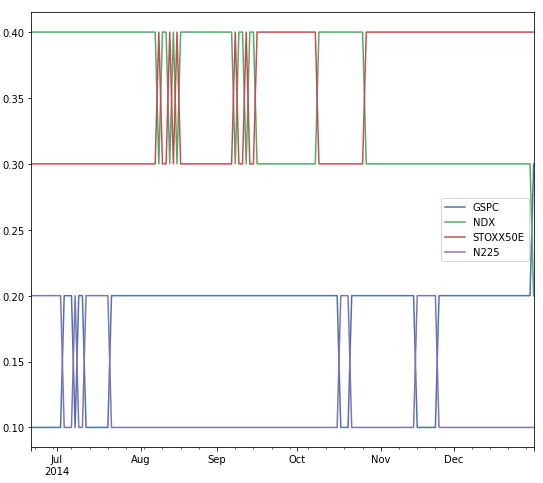
\includegraphics[width=7cm]{cap5/best_alloc_2014.png} }}%
	\subfloat[\centering  Temporal Convolutional Network allocation ]{{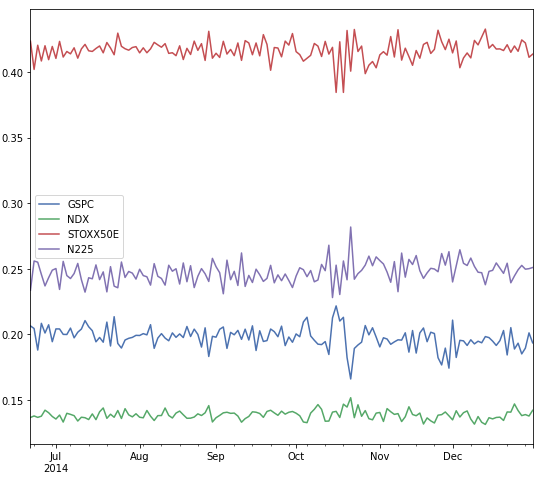
\includegraphics[width=7cm]{cap5/tcn_alloc_2014.png} }}%
	\qquad
	\subfloat[\centering  Long Short Term Memory Network allocation ]{{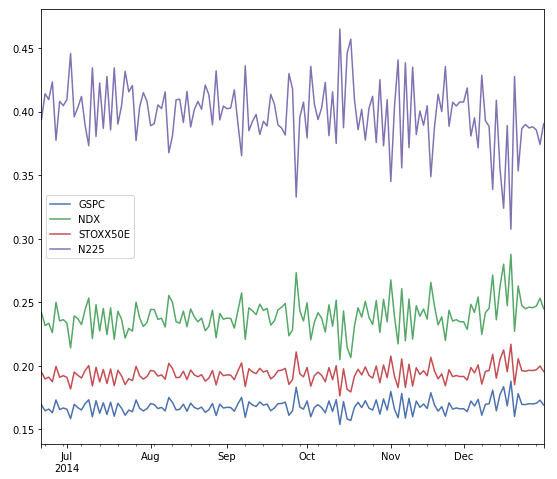
\includegraphics[width=7cm]{cap5/lstm_alloc_2014.png} }}%
	\subfloat[\centering Transformer allocation ]{{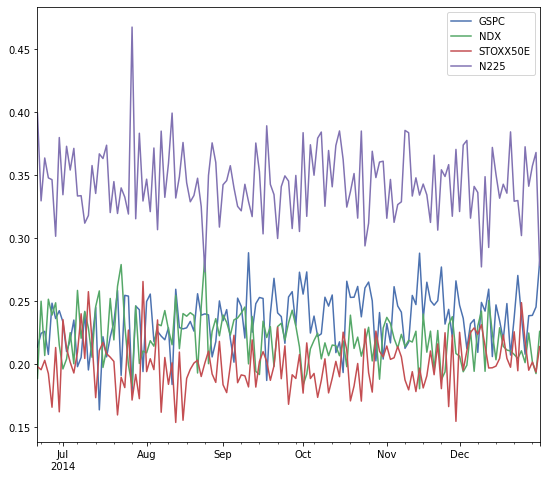
\includegraphics[width=7cm]{cap5/trasformer_alloc_2014.png} }}%
	\caption{Allocations generated from TCN, LSTM e Transformers}%
	\label{fig:allocation_comparison_architecture}%
\end{figure}

LSTM and Transformer perform poorly in the period shown because they do not invest enough in the EUROSTOXX 50, that is the 1st or 2nd best asset in the period. \\


Regularization techniques have been tried, by both inserting dropout in the TCN layer or a batch regularization layer after it. The results showed how these techniques bring little improvements if not worsen the results, therefore it have been decided to not use them in the final model.

\section{Hyperparameter selection}

\begin{figure}[H]
	\centering
	\subfloat[\centering Training loss]{{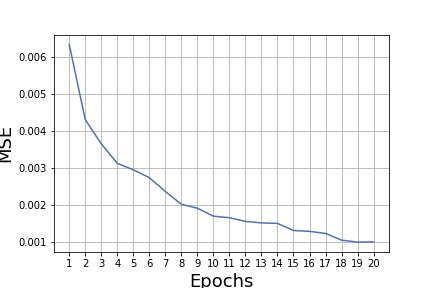
\includegraphics[width=7cm]{cap5/train_loss.png} }}%
	\subfloat[\centering  Validation loss ]{{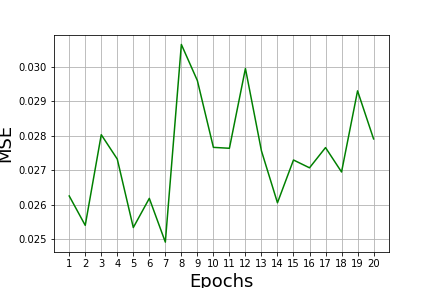
\includegraphics[width=7cm]{cap5/val_loss.png} }}%
	\caption{Model convergence: epochs and training/validation loss}%
	\label{fig:epochs_loss}%
\end{figure}

The TCN model converge as shown in the fig \ref{fig:epochs_loss} (a), the training loss decrease constantly during training. This is the minimization of the Empirical Risk discussed in chapter \ref{CH:theoryML}. Instead, TCN has problems of overfitting over six epochs, as shown in fig \ref{fig:epochs_loss} (b). Therefore we limited the number of epochs to five. This figure is the result of validating the model in the 2017 period. The reason why we have to limit ourselves to a so little epochs number can be explained by the fact we also have a little batch size (we use batches of dimension five). These two quantities are often related, as a small batch size make the network more sensible to small scale training data variations so less epochs are required to model these.



Models with a small window size, like 10 trading days, perform better in 2020 in a very volatile market phase, while models with a window size of 225 trading days perform better in the previous period 2013-2019 when the market was more stable. The window size of 125 trading days, around 6-7 full months, have shown to deliver the best results so far as it is a compromise between fast market change reaction and long term investment in reliable assets. \\

Regarding the other hyperparameters, a grid search using the TCN architecture have been carried out, with these ranges:
number of epochs = [5, 10], TCN filters = [8, 16, 32], convolution kernel size = [1, 2, 3], residual connection = enabled / disabled. \\
The results do not underline a trend, and it is impossible to say that a specific choice will for sure improve results. Still we kept the hyperparameters of the best results, namely 5 epochs, 32 filters, kernel size 3 and no residual connection.

\section{Selected model results}


A model has been selected following decisions described in the sections before.

\subsection{Generated allocation parametrization}
\label{allocation-parametrization}
We show that there is a certain degree of correlation between parameters of target allocation, i.e. Cumulative return, Sharpe ratio, and Volatility and the same parameters in the generated allocation, allowing risk control management. Table \ref{table:parametrization_1} shows the results of thirteen runs in the 2014 period of the selected model on different target allocation, the left part of the table, and the resulting performance parameters of the generated allocation (see the right part of the table). 

\hfill \break

\begin{table}[h]
	\resizebox{\textwidth}{!}{%
		\begin{tabular}{|l|l|l|
				>{\columncolor[HTML]{C0C0C0}}l |l|l|l|}
			\hline
			\begin{tabular}[c]{@{}l@{}}Target \\ return\end{tabular} & \begin{tabular}[c]{@{}l@{}}Target\\ Sharpe\end{tabular} & \begin{tabular}[c]{@{}l@{}}Target\\ std\end{tabular} &  & \begin{tabular}[c]{@{}l@{}}Generated\\ return\end{tabular} & \begin{tabular}[c]{@{}l@{}}Generated\\ sharpe\end{tabular} & \begin{tabular}[c]{@{}l@{}}Generated\\ std\end{tabular} \\ \cline{1-3} \cline{5-7} 
			30.1\%                                                   & 4.35                                                    & 0.40                                                 &  & 31.2\%                                                     & 4.44                                                       & 0.41                                                    \\ \cline{1-3} \cline{5-7} 
			44.9\%                                                   & 4.45                                                    & 0.59                                                 &  & 25.5\%                                                     & 3.02                                                       & 0.49                                                    \\ \cline{1-3} \cline{5-7} 
			39.2\%                                                   & 4.56                                                    & 0.50                                                 &  & 26.7\%                                                     & 3.37                                                       & 0.46                                                    \\ \cline{1-3} \cline{5-7} 
			43.1\%                                                   & 4.59                                                    & 0.55                                                 &  & 29.8\%                                                     & 3.88                                                       & 0.45                                                    \\ \cline{1-3} \cline{5-7} 
			35.4\%                                                   & 4.66                                                    & 0.44                                                 &  & 31.8\%                                                     & 4.36                                                       & 0.42                                                    \\ \cline{1-3} \cline{5-7} 
			43.6\%                                                   & 4.69                                                    & 0.54                                                 &  & 38.9\%                                                     & 4.28                                                       & 0.53                                                    \\ \cline{1-3} \cline{5-7} 
			40.8\%                                                   & 4.69                                                    & 0.51                                                 &  & 31.1\%                                                     & 3.78                                                       & 0.48                                                    \\ \cline{1-3} \cline{5-7} 
			37.6\%                                                   & 4.71                                                    & 0.46                                                 &  & 27.3\%                                                     & 3.72                                                       & 0.43                                                    \\ \cline{1-3} \cline{5-7} 
			41.6\%                                                   & 4.74                                                    & 0.51                                                 &  & 33.0\%                                                     & 3.82                                                       & 0.50                                                    \\ \cline{1-3} \cline{5-7} 
			42.8\%                                                   & 4.79                                                    & 0.52                                                 &  & 39.5\%                                                     & 4.38                                                       & 0.52                                                    \\ \cline{1-3} \cline{5-7} 
			42.8\%                                                   & 5.77                                                    & 0.43                                                 &  & 28.3\%                                                     & 3.99                                                       & 0.41                                                    \\ \cline{1-3} \cline{5-7} 
			63.3\%                                                   & 6.93                                                    & 0.53                                                 &  & 32.0\%                                                     & 4.14                                                       & 0.45                                                    \\ \cline{1-3} \cline{5-7} 
			62.2\%                                                   & 7.00                                                    & 0.52                                                 &  & 29.0\%                                                     & 3.92                                                       & 0.44                                                    \\ \hline
		\end{tabular}%
	}
	\caption[Target-Generated allocation performance]{Resulting performance parameters of generated allocation given parameters of target allocation in the 2014 period \label{table:parametrization_1}}
\end{table}

The correlation between these quantities is shown in Table \ref{table:parametrization_correlation}. Unfortunately the outcome is that only target and generated standard deviation are correlated (0.7) while return and Sharpe ratio are not.

\begin{table}[h]
	\resizebox{\textwidth}{!}{%
		\begin{tabular}{|c|l|l|l|l|l|l|}
			\hline
			\multicolumn{1}{|r|}{\textbf{}} & \multicolumn{1}{c|}{\textbf{\begin{tabular}[c]{@{}c@{}}Target \\ return\end{tabular}}} & \multicolumn{1}{c|}{\textbf{\begin{tabular}[c]{@{}c@{}}Target \\ Sharpe\end{tabular}}} & \multicolumn{1}{c|}{\textbf{\begin{tabular}[c]{@{}c@{}}Target \\ std\end{tabular}}} & \multicolumn{1}{c|}{\textbf{\begin{tabular}[c]{@{}c@{}}Generated \\ return\end{tabular}}} & \multicolumn{1}{c|}{\textbf{\begin{tabular}[c]{@{}c@{}}Generated \\ Sharpe\end{tabular}}} & \multicolumn{1}{c|}{\textbf{\begin{tabular}[c]{@{}c@{}}Generated \\ std\end{tabular}}} \\ \hline
			\textbf{Target return}          & 1.00                                                                                   & 0.89                                                                                   & 0.52                                                                                & -0.00                                                                                     & -0.08                                                                                     & 0.11                                                                                   \\ \hline
			\textbf{Target Sharpe}          & 0.89                                                                                   & 1.00                                                                                   & 0.08                                                                                & -0.06                                                                                     & 0.15                                                                                      & -0.24                                                                                  \\ \hline
			\textbf{Target std}             & 0.52                                                                                   & 0.08                                                                                   & 1.00                                                                                & 0.08                                                                                      & -0.49                                                                                     & 0.70                                                                                   \\ \hline
			\textbf{Generated return}       & -0.00                                                                                  & -0.06                                                                                  & 0.08                                                                                & 1.00                                                                                      & 0.72                                                                                      & 0.60                                                                                   \\ \hline
			\textbf{Generated Sharpe}       & -0.08                                                                                  & 0.15                                                                                   & -0.49                                                                               & 0.72                                                                                      & 1.00                                                                                      & -0.12                                                                                  \\ \hline
			\textbf{Generated std}          & 0.11                                                                                   & -0.24                                                                                  & 0.70                                                                                & 0.60                                                                                      & -0.12                                                                                     & 1.00                                                                                   \\ \hline
		\end{tabular}%
	}
	\caption[Performance correlation target-generated allocation]{Correlations between target and generated allocation parameters in the 2014 period \label{table:parametrization_correlation}}
\end{table}

This fact can be explained that often the target allocation are too hard for the network to match, either a too high return, where the network is unable to find out which components will perform better in the future, or a too low volatility, where the network is unable to predicting which components will have a lower volatility in the future. It exist a certain threshold over with the network stop performing better and instead perform worse than before, this explain some of the negative correlations.

\hfill \break

Instead, by relaxing the constraints and considering only a subset of the previous thirteen experiments we obtain far better results. We restrains the runs that have a cumulative return lower than $43\%$ and a standard deviation higher than $0.44$. We are left with six out of the original thirteen, that are still a significant sample and we again compute a correlation table shown in table \ref{table:parametrization_corr_2}.

\begin{table}[h]
	\resizebox{\textwidth}{!}{%
		\begin{tabular}{|c|l|l|l|l|l|l|}
			\hline
			\multicolumn{1}{|r|}{\textbf{}} & \multicolumn{1}{c|}{\textbf{\begin{tabular}[c]{@{}c@{}}Target \\ return\end{tabular}}} & \multicolumn{1}{c|}{\textbf{\begin{tabular}[c]{@{}c@{}}Target \\ Sharpe\end{tabular}}} & \multicolumn{1}{c|}{\textbf{\begin{tabular}[c]{@{}c@{}}Target \\ std\end{tabular}}} & \multicolumn{1}{c|}{\textbf{\begin{tabular}[c]{@{}c@{}}Generated \\ return\end{tabular}}} & \multicolumn{1}{c|}{\textbf{\begin{tabular}[c]{@{}c@{}}Generated \\ Sharpe\end{tabular}}} & \multicolumn{1}{c|}{\textbf{\begin{tabular}[c]{@{}c@{}}Generated \\ std\end{tabular}}} \\ \hline
			\textbf{Target return}          & 1.00                                                                                   & 0.52                                                                                   & 0.97                                                                                & 0.59                                                                                      & -0.02                                                                                     & 0.98                                                                                   \\ \hline
			\textbf{Target Sharpe}          & 0.52                                                                                   & 1.00                                                                                   & 0.29                                                                                & 0.78                                                                                      & 0.62                                                                                      & 0.55                                                                                   \\ \hline
			\textbf{Target std}             & 0.97                                                                                   & 0.29                                                                                   & 1.00                                                                                & 0.44                                                                                      & -0.20                                                                                     & 0.93                                                                                   \\ \hline
			\textbf{Generated return}       & 0.59                                                                                   & 0.78                                                                                   & 0.44                                                                                & 1.00                                                                                      & 0.79                                                                                      & 0.71                                                                                   \\ \hline
			\textbf{Generated Sharpe}       & -0.02                                                                                  & 0.62                                                                                   & -0.20                                                                               & 0.79                                                                                      & 1.00                                                                                      & 0.13                                                                                   \\ \hline
			\textbf{Generated std}          & 0.98                                                                                   & 0.55                                                                                   & 0.93                                                                                & 0.71                                                                                      & 0.13                                                                                      & 1.00                                                                                   \\ \hline
		\end{tabular}%
	}
	\caption{Correlations between target and generated allocation parameters on a restricted set of experiments \label{table:parametrization_corr_2}}
\end{table}

We can observe as the correlation between target and generated standard deviation is very high, it is easier for the network to predict future volatility than future returns. Still also the the target cumulative return and the generated cumulative return have a correlation coefficient of $0.59$ that is still significant. Ultimately, also the Sharpe ratio is correlated, as it is the ratio between the two previously mentioned quantities. 

\hfill \break

This indicates again that is possible to control the result allocation parameters and have risk control with the method researched and selected in this work.

Table \ref{t:selected_comparison_benchmarks} summarizes the selected model performance in comparison to the benchmarks: baseline algorithm, equally weighted, inverse volatility and risk parity benchmarks. 

\begin{table}[H]
	\begin{tabular}{|l|l|l|l|}
		\hline
		& \begin{tabular}[c]{@{}l@{}}June 2014\\ December 2014\end{tabular} & \begin{tabular}[c]{@{}l@{}}June 2016\\ December 2017\end{tabular} & \begin{tabular}[c]{@{}l@{}}June 2019\\ June 2020\end{tabular} \\ \hline
		Baseline algorithm & 1.4\%                                                             & 0.9\%                                                             & 8.0\%                                                         \\ \hline
		Equally allocation & 1.5\%                                                             & 1.6\%                                                             & 3.5\%                                                         \\ \hline
		Inverse volatility & 2.3\%                                                             & 4.5\%                                                             & 1.6\%                                                         \\ \hline
		Risk Parity        & 4.3\%                                                             & 3.3\%                                                             & 0.6\%                                                         \\ \hline
	\end{tabular}
	\caption[Performance difference between selected model and benchmarks methods]{Performance difference (cumulative return) between selected model and benchmarks methods \label{t:selected_comparison_benchmarks}}
\end{table}


What follows are sections describing the performance both in terms of cumulative return and of Sharpe ratio in the validation periods described in Chapter \ref{CH:Model_research}.

\subsection{2014 period}

\begin{figure}[H]
	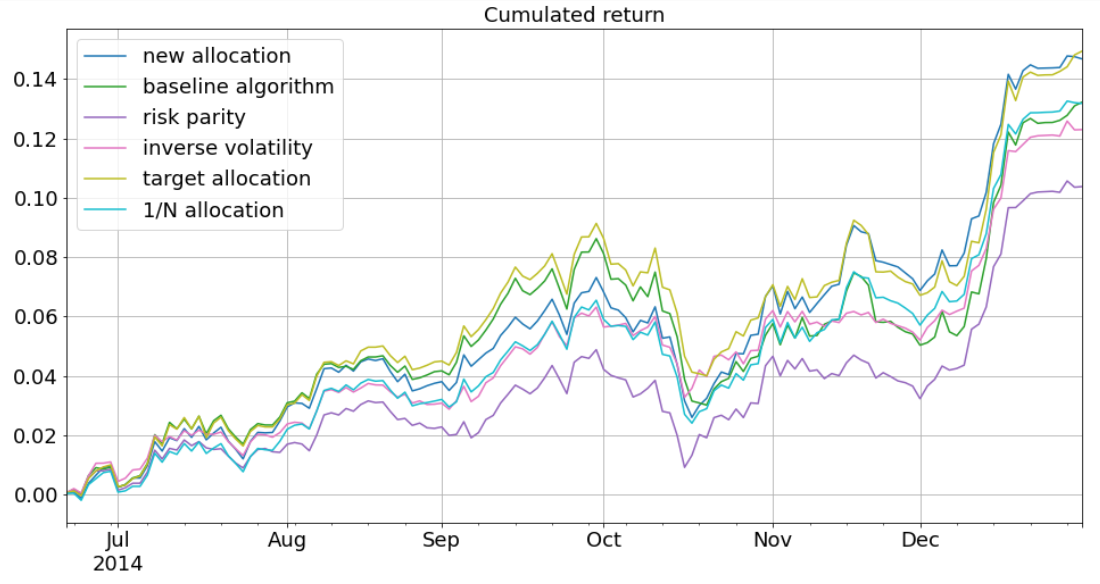
\includegraphics[width=\textwidth]{cap5/selected_cum_ret_2014.png}
	\caption{Selected model performance: Cumulative return, July-December 2014 }
	\label{fig:return_2014}
\end{figure}

2014 is the year were the network performs better among the analysed periods,  because it matches perfectly the target allocation in the second half of the time frame. Figure \ref{fig:return_2014} shows the cumulative return between July 2014 and December 2014. Our allocation method  performs better than all the benchmarks in consideration.\\


\begin{figure}[H]
	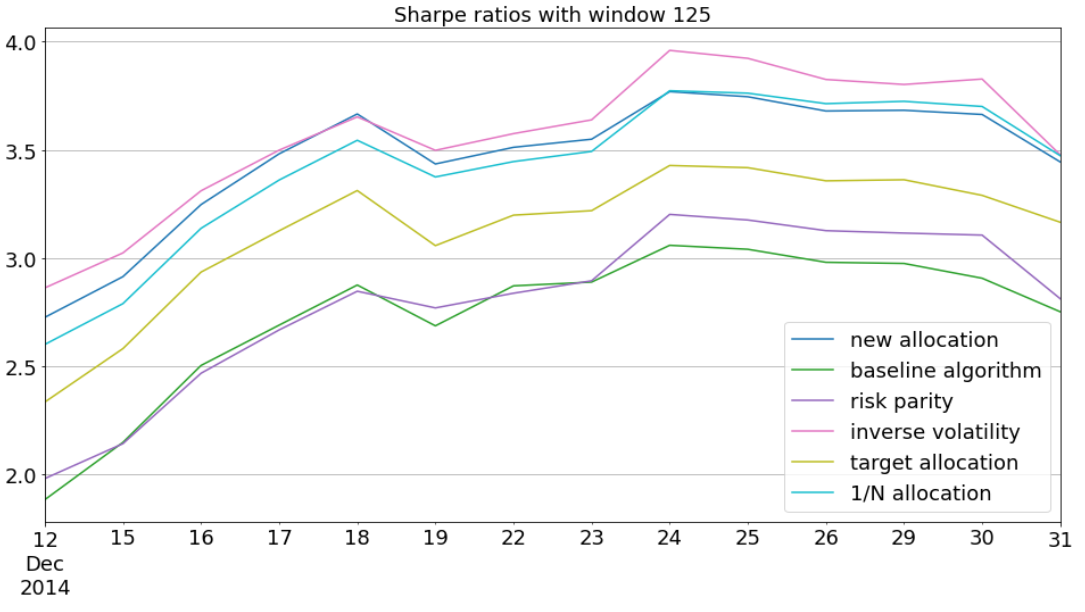
\includegraphics[width=\textwidth]{cap5/selected_sharpe_2014.png}
	\caption{Selected model performance: Sharpe ratio, December 2014 }
	\label{fig:sharpe_2014}
\end{figure}

In December 2014 period the Sharpe ratio is also considerably satisfactory, as seen in Figure \ref{fig:sharpe_2014}, as it is the highest between the benchmarks until December the 23rd and then it decreases only surpassed by inverse volatility and equally weighted methods.
The 2014 period is only 6 month long and 125 days are need to compute the Sharpe ratio, so as result we only have 31 days were the Sharpe ratio is computed, in December 2014. 

\newpage

\subsection{2016-2017 period}

\begin{figure}[H]
	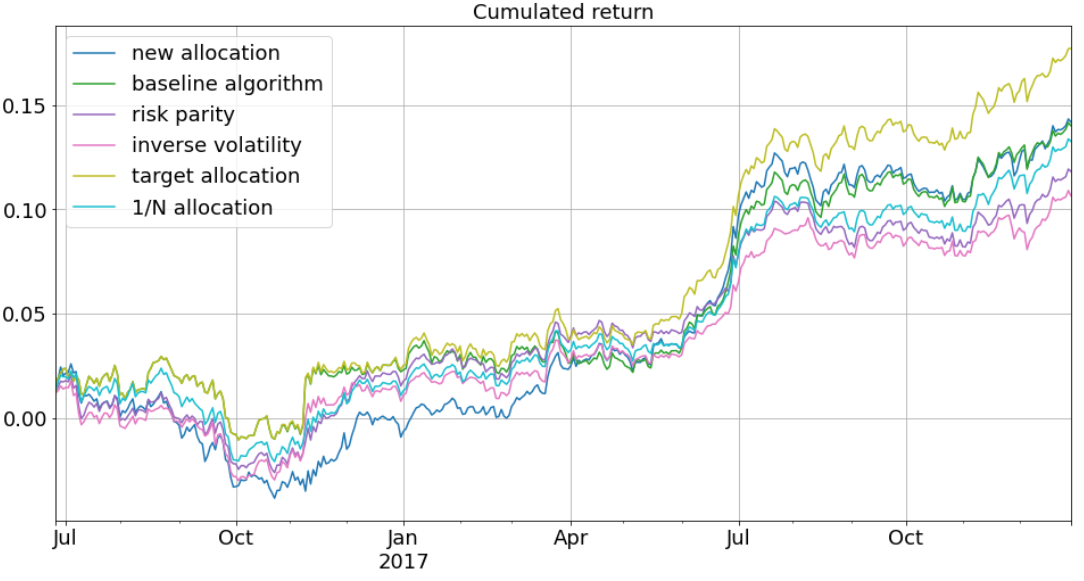
\includegraphics[width=\textwidth]{cap5/selected_cum_ret_2017.png}
	\caption{Selected model performance: Cumulative return, July 2016-November 2017 }
	\label{fig:return_2017}
\end{figure}

In the validation period July 2016 - November 2017 our method does not result in a higher cumulative return than the target allocation, like in the validation period July-December 2014, but it still outperforms all other benchmarks, as one can see in Figure \ref{fig:return_2017}.

\hfill \break

Sharpe ratio is shown between January and December 2017 in Figure \ref{fig:sharpe_2017}. Our method results in a Sharpe ratio in average with other benchmarks for most of the periods. It is under performing in the first months of January to March 2017 while it is superior between June and September 2017. However, it should be noted that also the target allocation does not perform better in term of Sharpe ratio with respect to the other benchmarks. This is because this allocation was created maximizing return and not Sharpe ratio.

\begin{figure}[H]
	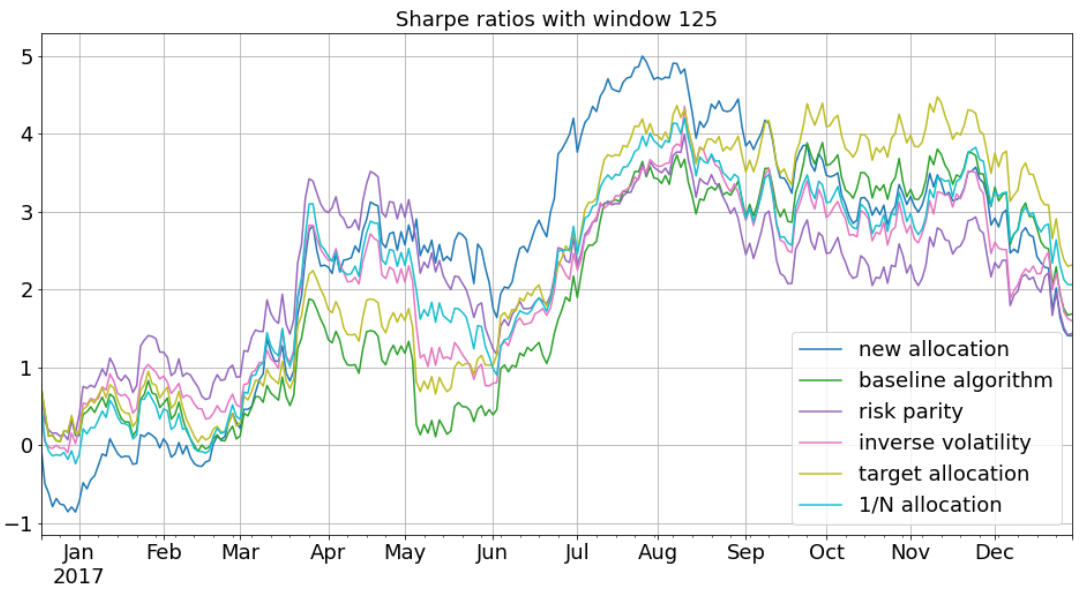
\includegraphics[width=\textwidth]{cap5/selected_sharpe_2017.png}
	\caption{Selected model performance: Sharpe ratio, January-December 2017 }
	\label{fig:sharpe_2017}
\end{figure}


\subsection{2019-2020 period}

\begin{figure}[H]
	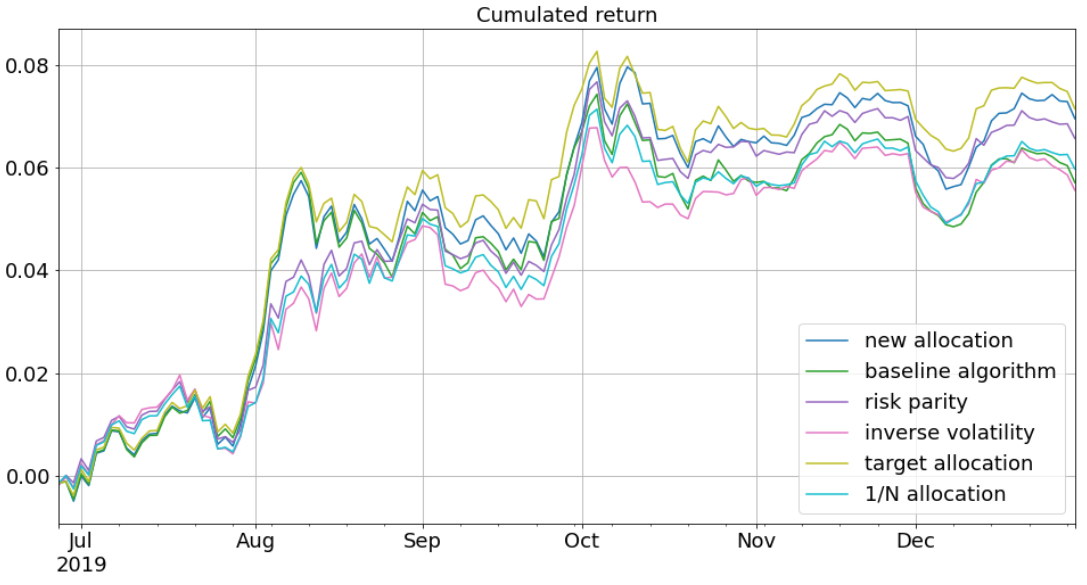
\includegraphics[width=\textwidth]{cap5/selected_cum_ret_2019.png}
	\caption{Selected model performance: Cumulative return, July 2019 - January 2020}
	\label{fig:return_2019}
\end{figure}

In the validation period 2019-2020 our method has two different phases so the cumulative return plot has been spitted in two parts for an easier comprehension. Figure \ref{fig:return_2019} shows the time frame July 2019 to January 2020 where the market was still growing and the benchmarks have all similar cumulative returns values. Still our model generates an allocation that in the end is superior to the baseline algorithm, the inverse volatility, and equally weighted allocations. \\

\begin{figure}[H]
	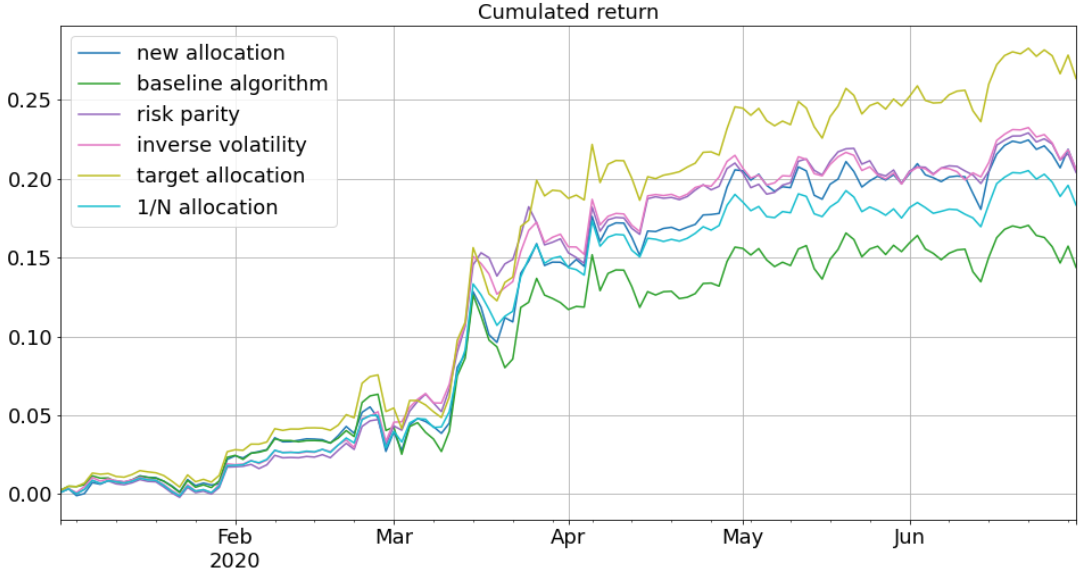
\includegraphics[width=\textwidth]{cap5/selected_cum_ret_2020.png}
	\caption{Selected model performance: Cumulative return, January-July 2020}
	\label{fig:return_2020}
\end{figure}



Within the time frame from January to July 2020, the 2020 stock market crash is included , but the strategy we used went short in that period so a surge in the cumulative return can be seen in March 2020 in Figure \ref{fig:return_2020}. Before March 2020 all the figures perform similarly but after they diverge significantly with our allocation method being superior to both baseline algorithm and equally weighted allocation and consistent with inverse volatility and risk parity. \\

\begin{figure}[H]
	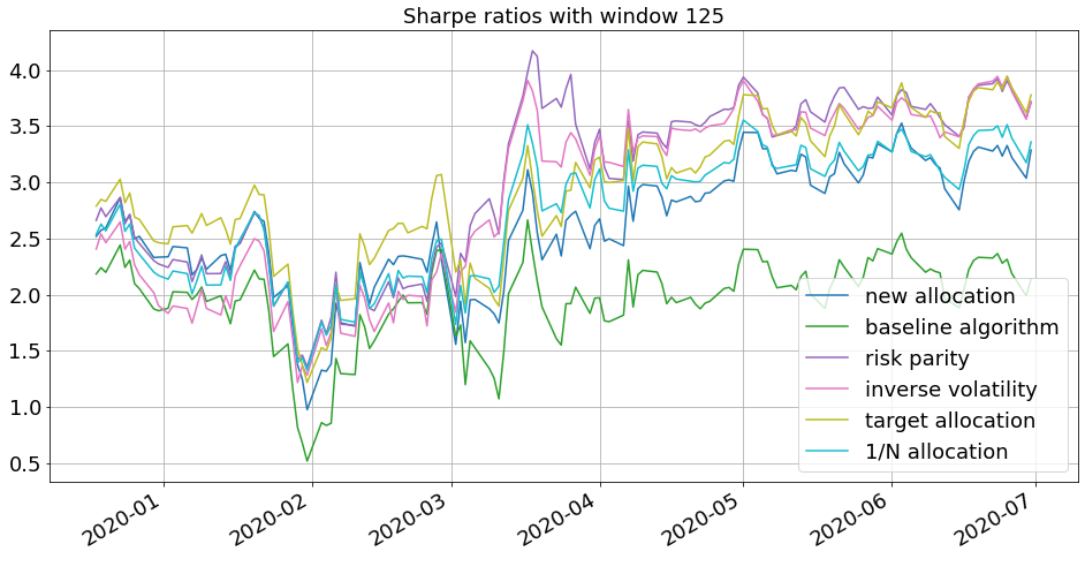
\includegraphics[width=\textwidth]{cap5/selected_sharpe_2020.png}
	\caption{Selected model performance: Sharpe ratio, January-July 2020}
	\label{fig:sharpe_2020}
\end{figure}



Sharpe ratio of the allocations in analysis for the period January to July 2020 can be seen in Figure \ref{fig:sharpe_2020}. Here our allocation method  performs poorly compared to the others and is inferior to most of them. Still it must be reminded that this allocation is not meant to have a high Sharpe ratio and it has a higher volatility compared to the other. We believe this explain this result.
